% !TeX spellcheck = en_GB
%
\documentclass[presentation]{beamer}
\mode<presentation>{\usetheme{AMSCesenaPurpleAndGold}}
\setbeamertemplate{bibliography item}{\insertbiblabel}
%%%%%%%%%%%%%%%%%%%%%%%%%%%%%%%%%%%%%%%%%%%%%%%%%%%%%%%%%%%%%%%%%%%%%%%%%%%%%%%%
%
\usepackage{jelia-2021-2pkt-talk}
%%%%%%%%%%%%%%%%%%%%%%%%%%%%%%%%%%%%%%%%%%%%%%%%%%%%%%%%%%%%%%%%%%%%%%%%%%%%%%%%
\title[Lazy Stream Manipulation in Prolog]{
    % same title of the presented paper
    Lazy Stream Manipulation in Prolog via Backtracking: The Case of \twopkt{}
}
%
% \subtitle{Extended Abstract}
%
% same authors order of the presented paper
\author[Ciatto et al.]{
	\emph{Giovanni Ciatto}$^{*}$ % empth the presenting author
	\and 
	Roberta Calegari$^{\dagger}$
	\and
	Andrea Omicini$^{*}$
}
%
\institute[UniBo]{
    $^{*}$Dipartimento di Informatica -- Scienza e Ingegneria (DISI)
    \\
    $^{\dagger}$Alma Mater Research Institute for Human-Centered Artificial Intelligence (Alma AI)
    \\
    \textsc{Alma Mater Studiorum} -- Università di Bologna
    \\
    \texttt{
        \{\emph{giovanni.ciatto}, roberta.calegari, andrea.omicini\}@unibo.it % emph the presenting author's email
    }
}
%
\date[JELIA, 2021]{
	$17^{th}$ Edition of the European Conference on
	\\
	Logics in Artificial Intelligence (JELIA 2021)
	\\
	May 17, 2021, Klagenfurt, Austria (Online Event)
}
%%%%%%%%%%%%%%%%%%%%%%%%%%%%%%%%%%%%%%%%%%%%%%%%%%%%%%%%%%%%%%%%%%%%%%%%%%%%%%%%
\AtBeginSection[]
{
%\\\\\\\\\\\\\\\\\\\\\
\begin{frame}<beamer>[c,noframenumbering]
\frametitle{Next in Line\ldots}
\tableofcontents[sectionstyle=show/shaded,subsectionstyle=hide]
\end{frame}
%\\\\\\\\\\\\\\\\\\\\\
}
\AtBeginSubsection[]
{
%\\\\\\\\\\\\\\\\\\\\\
\begin{frame}<beamer>[c,noframenumbering]
    \frametitle{Focus on\ldots}
	\mbox{~}
	\tableofcontents[currentsubsection,sectionstyle=shaded,subsectionstyle=show/shaded]
	\mbox{~}
\end{frame}
%\\\\\\\\\\\\\\\\\\\\\
}
%%%%%%%%%%%%%%%%%%%%%%%%%%%%%%%%%%%%%%%%%%%%%%%%%%%%%%%%%%%%%%%%%%%%%%%%%%%%%%%%
\begin{document}
%%%%%%%%%%%%%%%%%%%%%%%%%%%%%%%%%%%%%%%%%%%%%%%%%%%%%%%%%%%%%%%%%%%%%%%%%%%%%%%%

%\\\\\\\\\\\\\\\\\\\\\
\frame{\titlepage}
%\\\\\\\\\\\\\\\\\\\\\

%===============================================================================
\section{Motivation \& Context}
%===============================================================================

%\\\\\\\\\\\\\\\\\\\\\
\begin{frame}[allowframebreaks]{Context}
    
    \begin{itemize}
        \item We live in the data-driven AI era
        %
        \begin{itemize}
            \item pervasive need of processing wide amounts of data
            \item[eg] coming form sensors, smart devices, social networks etc.
        \end{itemize}
        
        \bigskip
        
        \item Stream processing is the preferred way towards \alert{scalability}
        %
        \begin{itemize}
            \item streams as possibly \alert{unlimited FIFO queues} of data
            \item either \emph{cold} (a.k.a. \alert{pull}) or \emph{hot} (a.k.a. \alert{push}) depending data \alert{generation}
            \item processing does not require loading \emph{all} data in memory
            \item support for \alert{lazy} manipulation of data
        \end{itemize}
        
        \framebreak
        
        \item Main-stream programming languages are blending FP with OOP
        %
        \begin{itemize}
            \item[$\rightarrow$] cascades of higher-order functions as stream-processing pipelines
            \item[eg] map, flat map, filter, fold, reduce, etc 
        \end{itemize}
        
        \bigskip
        
        \item Plenty of technologies for stream processing \alert{in the large}
        %
        \begin{itemize}
            \item featuring advancend, time-related operators 
            \item[eg] Kafka, Flink, Spark, Storm, etc.
        \end{itemize}
        
    \end{itemize}
\end{frame}
%\\\\\\\\\\\\\\\\\\\\\

%\\\\\\\\\\\\\\\\\\\\\
\begin{frame}[c]{Motivation}
    \begin{block}{Question 1}
        \centering
        What is the role of LP in stream processing?
    \end{block}
    %
    \begin{itemize}
        \item LP as a means to express \alert{complex event processing} \ccite{AnicicFRSSS10,AnicicRFS12}
        \item \alert{ASP} as a means to reason over \emph{hot} streams \ccite{BeckEB17,Beck2018}
    \end{itemize}

    \vfill

    \begin{block}{Question 2}
        \centering
        What is the role of \emph{Prolog} in stream processing?
    \end{block}
    %
    \begin{itemize}
        \item[$\uparrow$] this is the focus of this work
    \end{itemize}
\end{frame}
%\\\\\\\\\\\\\\\\\\\\\

%\\\\\\\\\\\\\\\\\\\\\
\begin{frame}{Contributions of this Work}

    \begin{enumerate}
        \item We show that Prolog \emph{already} supports lazy stream manipulation
        %
        \begin{itemize}
            \item as Prolog solvers can be intended as \alert{prosumers} of data
        \end{itemize}
        
        \vfill
        
        \item We propose a notion of \alert{generator} aimed letting solvers:
        %
        \begin{itemize}
            \item lazily consume streams of data from the external world
        \end{itemize}

        \vfill  
        
        \item We sketch \alert{state-machine-based} design for Prolog solvers
        %
        \begin{itemize}
            \item aimed at supporting the aforementioned notion of \alert{generator}
            \item without affecting its syntax, nor its semantics
        \end{itemize}

        \vfill  

        \item We demonstrate how generators can be exploited in practice
        %
        \begin{itemize}
            \item[eg] letting Prolog invoke external solvers and lazily consume their responses
            \item via the \twopkt{} technology \ccite{homepage2PKt}
        \end{itemize}
    \end{enumerate}

\end{frame}
%\\\\\\\\\\\\\\\\\\\\\

%===============================================================================
\section{Logic Solvers as Streams Prosumers}
%===============================================================================

%\\\\\\\\\\\\\\\\\\\\\
\begin{frame}[allowframebreaks]
\frametitle{Logic Solvers as Data \textbf{Producers}}

    % \begin{columns}
    %     \begin{column}{.48\linewidth}
    %         \onslide<1>{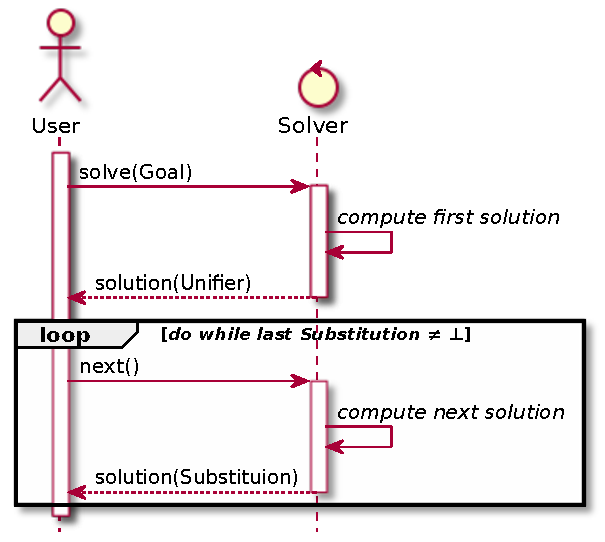
\includegraphics[width=\linewidth]{img/stateful-solver.pdf}}
    %     \end{column}
    %     \begin{column}{.04\linewidth}
    %         \onslide<1->{$\rightarrow$}
    %     \end{column}
    %     \begin{column}{.48\linewidth}
    %         \onslide<2>{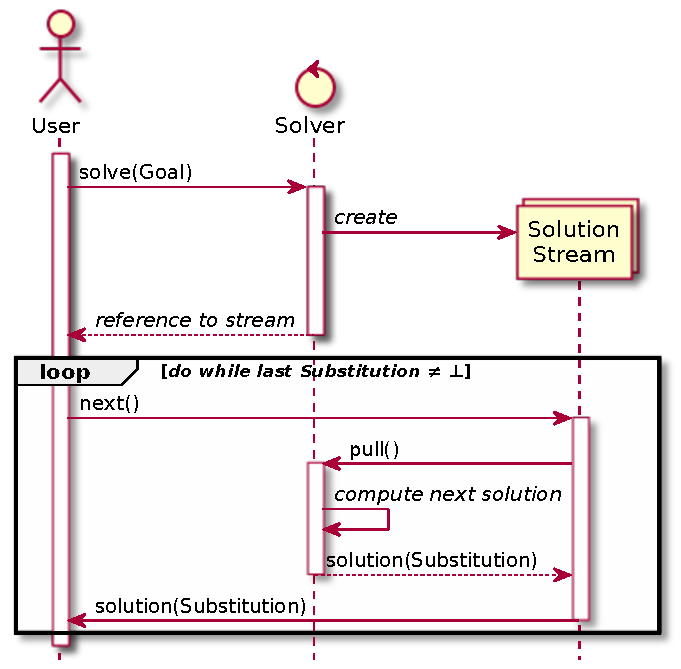
\includegraphics[width=\linewidth]{img/streamful-solver.pdf}}
    %     \end{column}
    % \end{columns}

    % \vfill

    % \begin{itemize}
    %     \item<1-> Logic solvers naturally support the \alert{lazy} exploration of solution spaces
    %     %
    %     \begin{itemize}
    %         \item[eg] Prolog solvers, via \alert{backtracking}
    %     \end{itemize}

    %     \item<2> They can be interpreted as \alert{producers} of \emph{cold} streams
    % \end{itemize}

    \begin{center}
        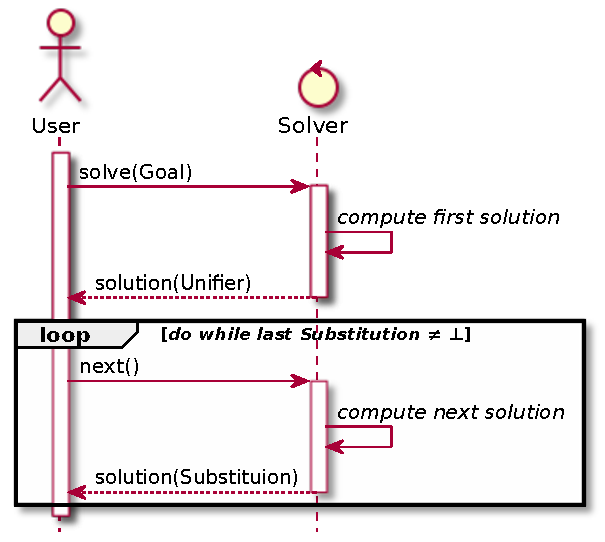
\includegraphics[width=.5\linewidth]{img/stateful-solver.pdf}
    \end{center}
    %
    \begin{itemize}
        \item Logic solvers naturally support the \alert{lazy} exploration of solution spaces
        %
        \begin{itemize}
            \item[eg] Prolog solvers, via \alert{backtracking}
            \item \alert{solutions} are generated on the fly, upon \alert{users'} requests
        \end{itemize}
    \end{itemize}
    
    \framebreak

    \begin{center}
        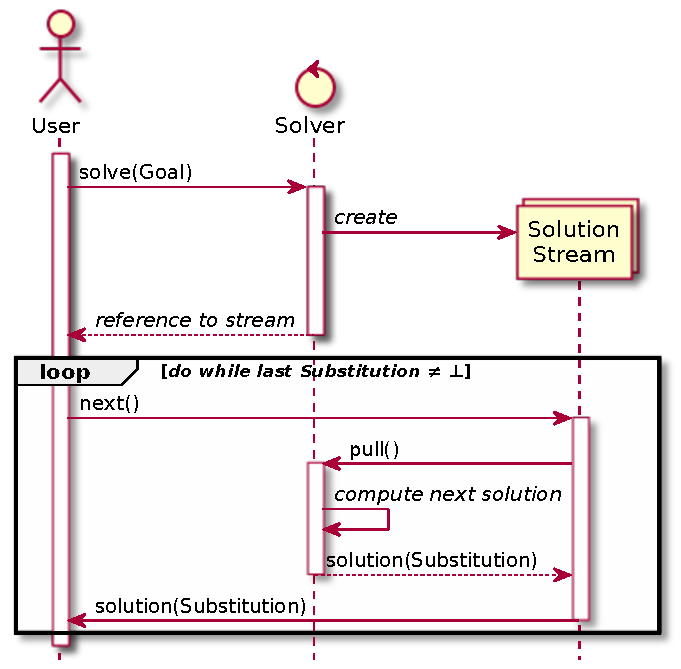
\includegraphics[width=.5\linewidth]{img/streamful-solver.pdf}
    \end{center}
    %
    \begin{itemize}
        \item[$\rightarrow$] They can be conceived as \alert{producers} of \emph{cold} streams of solutions
    \end{itemize}

\end{frame}
%\\\\\\\\\\\\\\\\\\\\\

%\\\\\\\\\\\\\\\\\\\\\
\begin{frame}%[allowframebreaks]
    \frametitle{Logic Solvers as Data \textbf{Consumers}}
    
    \begin{center}
        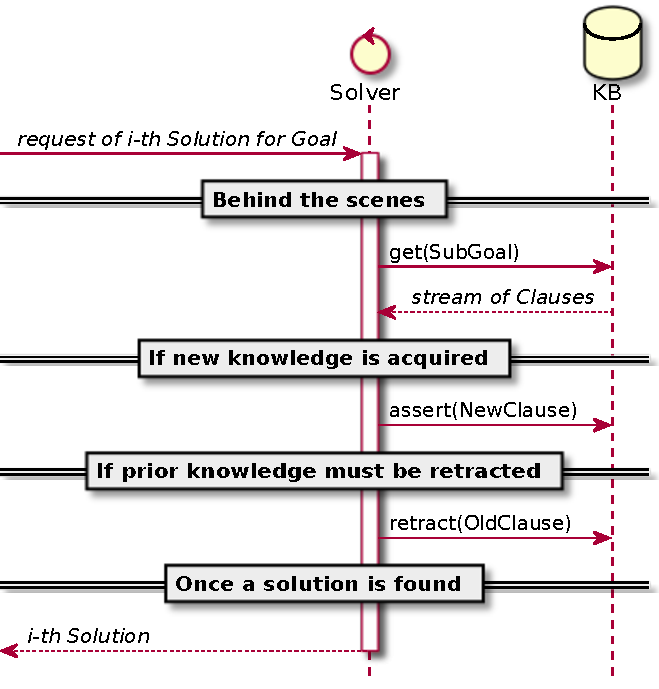
\includegraphics[width=.4\linewidth]{img/streamful-kb.pdf}
    \end{center}
    %
    \begin{itemize}
        \item Logic solvers naturally support the \alert{lazy} retrieval of clauses from KB
        \item[$\rightarrow$] They can be conceived as \alert{consumers} of \emph{hot} streams of clauses
    \end{itemize}
    
\end{frame}
%\\\\\\\\\\\\\\\\\\\\\

%===============================================================================
\section{Generators}
%===============================================================================

%\\\\\\\\\\\\\\\\\\\\\
\begin{frame}%[allowframebreaks]
    \frametitle{Why Generators}

    \begin{alertblock}{Problem}
        \begin{itemize}
            \item How to make logic solvers \alert{cold} strems consumers? 
        \end{itemize}
    \end{alertblock}

\end{frame}
%\\\\\\\\\\\\\\\\\\\\\

%\\\\\\\\\\\\\\\\\\\\\
\begin{frame}[allowframebreaks]
    \frametitle{Generators}

    \begin{columns}
        \begin{column}{.6\linewidth}
            \begin{exampleblock}{Concept}
                \begin{enumerate}\small
                    \item Some predicates are \alert{generators}
                    \item Solving (sub-)goals matching them means:
                    %
                    \begin{itemize}\scriptsize
                        \item lazily consuming solutions 
                        \item generated by some external entity, on the fly
                        \item whevener requested by the resolution process
                    \end{itemize}
                \end{enumerate}
            \end{exampleblock}        
        \end{column}
        \hfill
        \begin{column}{.4\linewidth}
            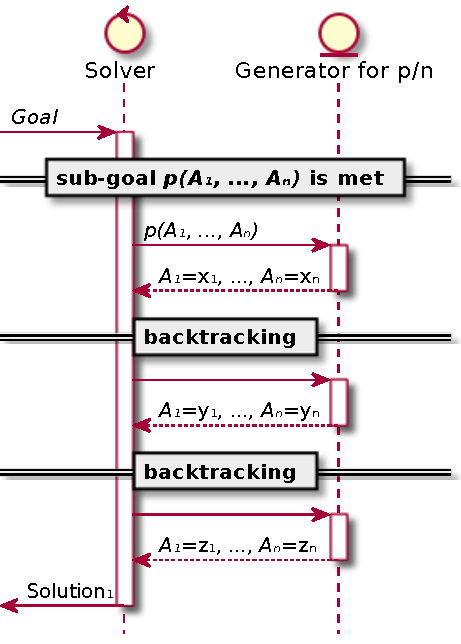
\includegraphics[width=\linewidth]{img/solver-generator.pdf}
        \end{column}
    \end{columns}

    \framebreak

    \begin{center}
        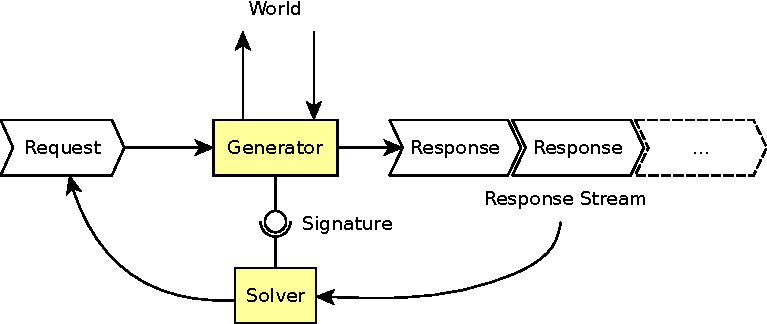
\includegraphics[width=.6\linewidth]{img/generator.pdf}
    \end{center}

    \begin{block}{Definition (informal)}
        \begin{itemize}
            \item Generator as \alert{functions} of the form: $Request \rightarrow Response^*$
            %
            \begin{description}
                \item[Requests] carry variables + execution context
                \item[Responses] carry variables assignments
            \end{description}
            \item accessible by \alert{signature} (functor/arity)
        \end{itemize}
    \end{block}

\end{frame}
%\\\\\\\\\\\\\\\\\\\\\

\subsection{Generators in Prolog}

%\\\\\\\\\\\\\\\\\\\\\
\begin{frame}[allowframebreaks]
    \frametitle{State-Machine for Prolog, supporting Generators}

    \begin{itemize}
        \item State-Machine for Prolog, proposed in \ccite{tuprolog-sac08}
        %
        \begin{itemize}
            \item extended to support \alert{generators}
        \end{itemize}
    \end{itemize}

    \begin{center}
        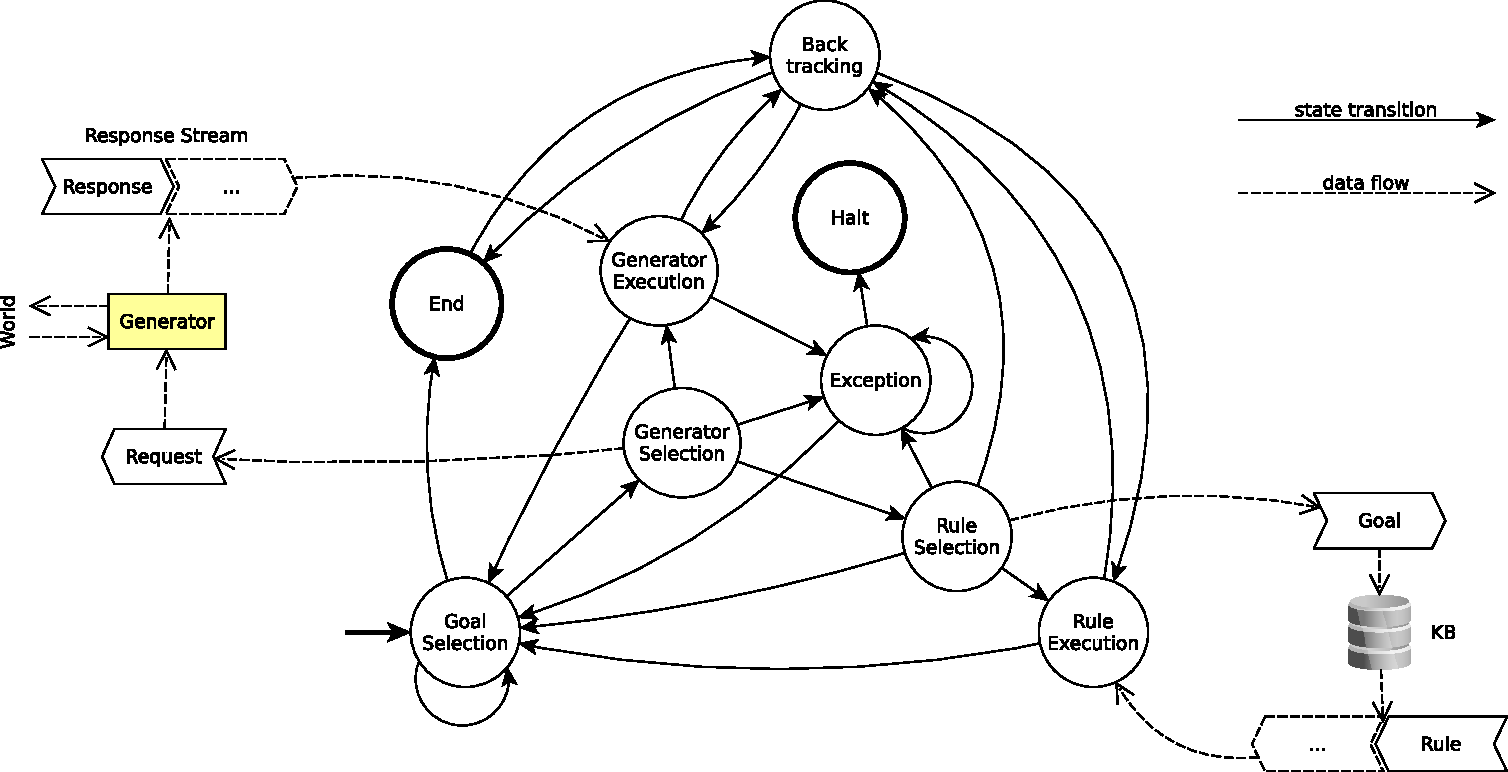
\includegraphics[width=.8\linewidth]{img/2p-fsa-dataflow.pdf}
    \end{center}

    \begin{block}{Locations}
        \begin{description}\small
            \item[\textsf{Goal Selection}] selects the next (sub-)goal to be proved

            \item[\textbf{\textsf{Generator Selection}}] looks for a generator to solve the selected (sub-)goal
            
            \item[\textbf{\textsf{Generator Execution}}] if some is found, the $1^{st}$ response is consumed
        
            \item[\textsf{Rule Selection}] if no primitive is selected, some rule is looked for instead
            
            \item[\textsf{Rule Execution}] if a rule is found, resolution proceeds 
            
            \item[\textsf{Backtracking}] if no rule is found, the sub-goal is considered failed 
            %
            \begin{itemize}
                \item resolution may then go back to \textsf{Generator/Rule Selection}
            \end{itemize}

            \item[\ldots]
        \end{description}
    \end{block}

    \hfill\hint{formalization attempt here: \url{https://github.com/tuProlog/2pkt-state-machine}}

\end{frame}
%\\\\\\\\\\\\\\\\\\\\\

\section{Case study: TSP in Prolog}


%\\\\\\\\\\\\\\\\\\\\\
\begin{frame}%[allowframebreaks]
\frametitle{\twopkt{} + Google OR-Tools}
    \begin{columns}
        \begin{column}{.62\linewidth}
            \begin{itemize}
                \item \alert{\twopkt{}}: open-source technolgy for LP \ccite{homepage2PKt}
                %
                \begin{itemize}
                    \item supporing Prolog + generators
                \end{itemize}

                \bigskip

                \item \alert{OR-Tools}: Google's open-source library for optimization \ccite{ortools}
                
                \bigskip

                \item Generator for \alert{\texttt{tsp/3}} predicate\footnotemark
                %
                \begin{itemize}
                    \item Prolog computing TSP via OR-Tools
                \end{itemize}

            \end{itemize}
        \end{column}
        \begin{column}{.38\linewidth}
            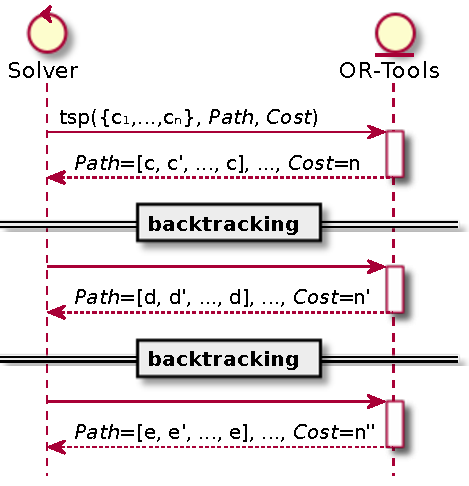
\includegraphics[width=\linewidth]{img/or-tools.pdf}
        \end{column}
    \end{columns}

    \footnotetext{cf. \url{https://github.com/tuProlog/ortools-tsp-example}}
\end{frame}
%\\\\\\\\\\\\\\\\\\\\\

\section{Conclusions \& future works}

%\\\\\\\\\\\\\\\\\\\\\
\begin{frame}%[allowframebreaks]
\frametitle{Conclusions \& future works}

\begin{block}{Summing up, in this work we}
    \begin{itemize}
        \item propose generators for manipulating cold streams via logic solvers
        \item sketch their semantics in Prolog via a state-machine
        \item demonstrate the feasibility of the approach via \twopkt{} + OR-Tools
    \end{itemize}
\end{block}

\begin{exampleblock}{Future works}
    \begin{itemize}
        \item Extend the framework to support side-effects
        \item Extend the framework to support time and hot streams
        \item Provide semantics for non-Prolog solvers
    \end{itemize}
\end{exampleblock}

\end{frame}
%\\\\\\\\\\\\\\\\\\\\\

%===============================================================================
\section*{}
%===============================================================================
\frame{\titlepage}

%===============================================================================
\section*{\bibname}
%===============================================================================

\setbeamertemplate{page number in head/foot}{}
%\\\\\\\\\\\\\\\\\\\\\
\begin{frame}[t,allowframebreaks,noframenumbering]\frametitle{\refname}
% \begin{frame}[c]\frametitle{\refname}
	\footnotesize
%	\scriptsize
    \bibliographystyle{plain}
	\bibliography{jelia-2021-2pkt-talk}
\end{frame}
%\\\\\\\\\\\\\\\\\\\\\

%%%%%%%%%%%%%%%%%%%%%%%%%%%%%%%%%%%%%%%%%%%%%%%%%%%%%%%%%%%%%%%%%%%%%%%%%%%%%%%%
\end{document}
%%%%%%%%%%%%%%%%%%%%%%%%%%%%%%%%%%%%%%%%%%%%%%%%%%%%%%%%%%%%%%%%%%%%%%%%%%%%%%%%
